\documentclass{article}[18pt]
\usepackage{../../../../../format}
\lhead{MCS - Logic and Discrete Structures}


\begin{document}
\begin{center}
\underline{\huge Week 5 Practical}
\end{center}
\section{Question 1}
\textit{On an island there are knights who always tell the truth and knaves who always lie. You meet three people: A, B, and C.
\begin{itemize}
\item A says: “I am a knave and B is a knight.”
\item B says: “Exactly one of the three of us is a knight.”
\end{itemize}}
A's statement must be at least partly false as a knight could never say they were a knave, therefore both A and B must be knaves. Because of this B's statement must be false, so C cannot be a knight, and so must also be a knave.\\
\\
A,B and C are knaves.
\section{Question 2}
\textit{The logical connective NAND is such that:
\begin{center}
	p NAND q is \textbf{false} if, and only if, p and q are both \textbf{true}.
\end{center}
Prove that p NAND (q NAND r) and (p NAND q) NAND r are not equivalent.}
$$p \ NAND \ (q \ NAND \ r)\neq (p \ NAND \ q) \ NAND \ r$$
$$\lnot(p\land\lnot(q\land r))\neq \lnot(r\land\lnot(p\land q))$$
Remove Negation, Apply De Morgan's to both sides, then remove negation again.
$$\lnot p\lor(q\land r)\neq \lnot r\land(p\land q)$$
If p is true, then for the LHS to be true, both q and r must be true. However, if r is true the RHS cannot be true.
\section{Question 3}
\textit{Show that the following propositional formulae are tautologies without using truth tables:}
$$(\lnot q\land(p\Rightarrow q))\Rightarrow\lnot q$$
This could only be false if the LHS was true and the RHS false. For this q would have to be true. However, if q was true then $\lnot q\land (p\Rightarrow q)$ could never be true. Therefore, this is a tautology.
$$((p\lor q)\land\lnot p)\Rightarrow q$$
For the statement to be false, q must be false and the LHS true.\\
If q is false then the LHS simplifies to $p\land\lnot p$ which can never be true, so the statement is a tautology.
\section{Question 4}
Show that $(a\lor c)\land (b\Rightarrow c)\land (c\Rightarrow a)$ and $(b\Rightarrow c)\land a$ are logically equivalent without using truth tables.\\
$(a\lor c)\land (c\land a)$ is true whenever a is true as $c\land a$ can only be false when a is false and $a\lor c$ is trivially true when a is true.\\
Therefore $(a\lor c)\land (c\land a)$ can be simplified to a, and so the whole RHS simplified to $(b\Rightarrow c)\land a$, which is equal to the RHS.
\newpage
\section{Question 5}
\textit{The logical connective NAND is such that:
	\begin{center}
		p NAND q is \textbf{false} if, and only if, p and q are both \textbf{true}.
	\end{center}
and the logical connective NOR is such that
	\begin{center}
		p NOR q is \textbf{true} if, and only if, p and q are both \textbf{flase}.
	\end{center}
Write p NAND q and p NOR q using only $\land \lor$ and $\lnot$}\\
p NAND q = $\lnot(p \land q)$\\
p NOR q= $\lnot(p\lor q)$\\
\\
\textit{Write $p \lor q, p \land q, and \lnot p$ using only NAND and NOR}\\
$p\land q$ = (p NOR p) NOR (q NOR q)\\
$p\lor q$ = (p NOR q) NOR (p NOR q)\\
$\lnot p$ = p NOR p

\section{Question 6}
Find a propositional formula involving only the logical connective NOR that
is logically equivalent to X $\Rightarrow$ Y .\\
\\
$p \Rightarrow q$ is equivalent to $\lnot p\lor q$, and that is equivalent to :
\begin{center}
((p NOR p)NOR q)NOR ((p NOR p)NOR q)
\end{center}
\section{Question 7 - Conjunctive Normal Form}
\textit{Which of the following propositional formulae are satisfiable (that is, are such that there is a satisfying truth assignment)?}
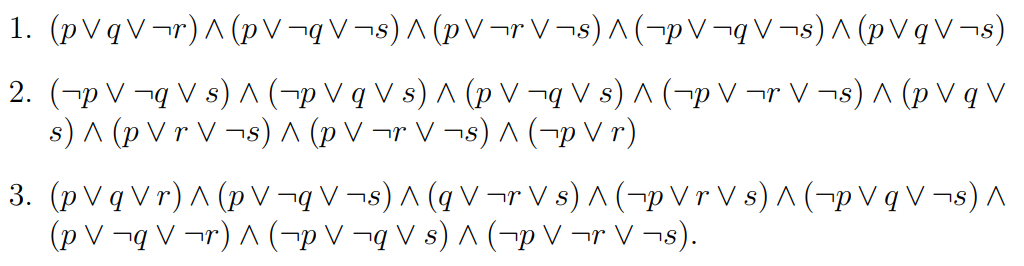
\includegraphics[width=15cm]{Q7.png}\\
1 is satisfiable as all but one of the brackets contain $\lnot s$, so when s is false, all of those brackets are satisfied, then the first bracket can be satisfied with either p true, q true or r false.\\
\\
2 is not satisfiable as p being assigned true or false satisfies half the brackets. However, each of the remaining letters can only satisfy one more bracket with either of their truth assignment. This means that one bracket will always remain unsatisfied.\\
\\
3 is satisfied by the truth assignment p false, q false, r true, s true
\section{Question 8 - Conjunctive normal form}
\textit{Reduce the following formulae $\varphi$ to conjunctive normal form by first reducing $\lnot \varphi$ to disjunctive normal form using truth tables.}\\
\\
$\mathbf{((p\land\lnot q)\lor r)\Rightarrow (\lnot p \land \lnot r)}$\\
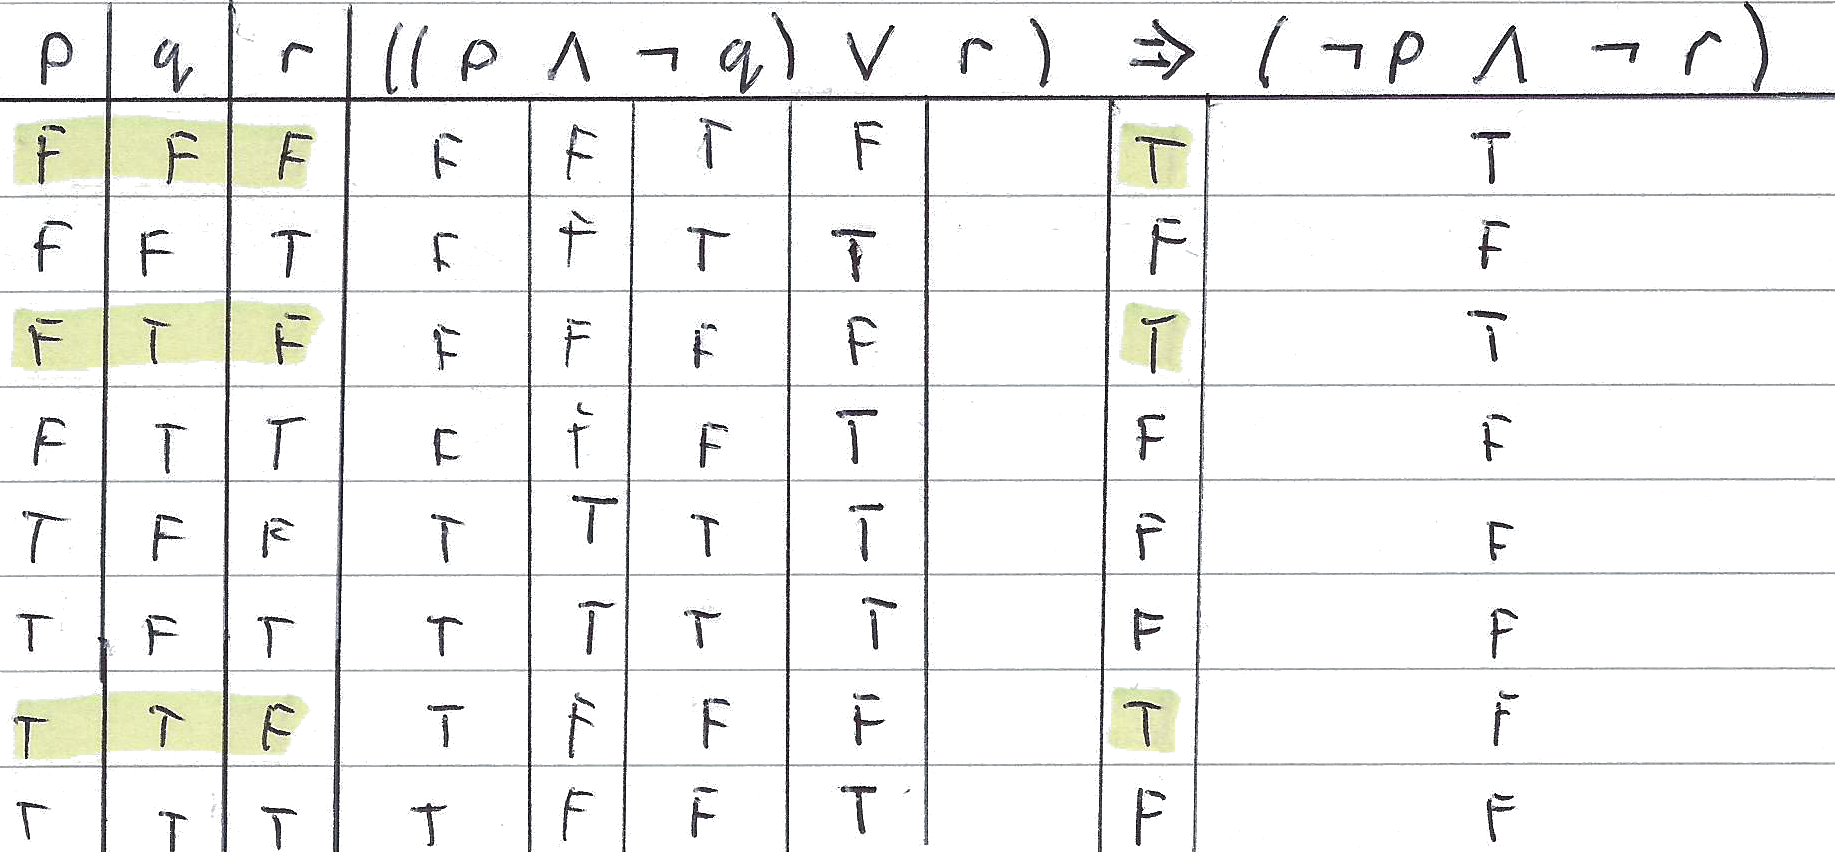
\includegraphics[width=10cm]{Truth_Table.png}
\\
$\lnot \varphi$ is equivalent to:
$$(\lnot p\land\lnot q\land r)\lor(\lnot p\land q\land r)\lor (p\land\lnot q\land\lnot r)\lor(p\land\lnot q\land r)\lor (p\land q\land r)$$
Hence, $\varphi$ is equivalent to
$$(p\lor q\lor \lnot r)\land( p\lor \lnot q\lor \lnot r)\land (\lnot p\lor q\lor r)\land(\lnot p\lor q\lor\lnot r)\land (\lnot p\lor\lnot q\land \lnot r)$$
\\
\\
$((p\land (q\Rightarrow r))\Rightarrow s)$\\
$\lnot \varphi$ is equivalent to
$$(p\land\lnot q\land\lnot r\land\lnot s)\lor (p\land\lnot q\land r\land\lnot s)\lor (p\land q\land r\land\lnot s)$$
Hence, $\varphi$ is equivalent to
$$(\lnot p\lor q\lor r\lor s)\land (\lnot p\lor q\lor \lnot r\lor s)\land (\lnot p\lor \lnot q \lor\lnot r \lor s)$$
\end{document}